\documentclass[a4paper,12pt,twoside,openright,titlepage]{book}

%Additional packages
\usepackage[utf8]{inputenc}
\usepackage[T1]{fontenc}
\usepackage[dutch,english]{babel}
\usepackage{imakeidx}
\usepackage{syntonly}
\usepackage[official]{eurosym}
%\usepackage[graphicx]
\usepackage{graphicx}
\graphicspath{ {./images/} }
\usepackage{float}
\usepackage{xurl}
\usepackage{hyperref}
\hypersetup{colorlinks=true, linkcolor=blue, citecolor=blue, filecolor=blue, urlcolor=blue, pdftitle=, pdfauthor=, pdfsubject=, pdfkeywords=}
\usepackage{tabularx}
\usepackage[table]{xcolor} % Table colors
\usepackage{scrextend}
\addtokomafont{labelinglabel}{\sffamily}
\usepackage{listings}
\usepackage{adjustbox}
\usepackage{color}

% Define colors
\definecolor{ashgrey}{rgb}{0.7, 0.75, 0.71}

% Listing style
\lstset{
  backgroundcolor=\color{ashgrey}, % choose the background color; you must add \usepackage{color} or \usepackage{xcolor}; should come as last argument
  basicstyle=\footnotesize,        % the size of the fonts that are used for the code
  breakatwhitespace=true,          % sets if automatic breaks should only happen at whitespace
  breaklines=true,                 % sets automatic line breaking
  extendedchars=true,              % lets you use non-ASCII characters; for 8-bits encodings only, does not work with UTF-8
  frame=single,	                   % adds a frame around the code
  rulecolor=\color{black},         % if not set, the frame-color may be changed on line-breaks within not-black text (e.g. comments (green here))
  keepspaces=true,                 % keeps spaces in text, useful for keeping indentation of code (possibly needs columns=flexible)
  columns=fullflexible,		   % make copy and paste possible
  showstringspaces=false,          % if true show spaces in strings adding particular underscores
  showspaces=false,                % if true show spaces everywhere adding particular underscores; it does not override 'showstringspaces'
}

% Uncomment for production
% \syntaxonly

% Style
\pagestyle{headings}

% Turn on indexing
\makeindex[intoc]

% Define document
\author{D. Leeuw}
\title{Elektrische componenten}
\date{\today\\v.0.8.0}

\begin{document}
\selectlanguage{dutch}

\maketitle

\copyright\ 2024 Dennis Leeuw\\

\begin{figure}

\includegraphics[width=0.3\textwidth]{CC-BY-SA-NC.png}
\end{figure}

\bigskip

Dit werk is uitgegeven onder de Creative Commons BY-NC-SA Licentie en laat anderen toe het werk te kopi\"eren, distribueren, vertonen, op te voeren, en om afgeleid materiaal te maken, zolang de auteurs en uitgever worden vermeld als maker van het werk, het werk niet commercieel gebruikt wordt en afgeleide werken onder identieke voorwaarden worden verspreid.


%%%%%%%%%%%%%%%%%%%
%%% Introductie %%%
%%%%%%%%%%%%%%%%%%%

\frontmatter
\chapter{Over dit Document}
\input{src/OverDitDocument}
\input{src/DocChanges}

%%%%%%%%%%%%%%%%%
%%% De inhoud %%%
%%%%%%%%%%%%%%%%%
\tableofcontents

\mainmatter
\chapter{Inleiding}
Dit hoofdstuk bevat een aantal componenten die in de elektronica\index{Componenten}\index{Elektronische componenten} gebruikt worden om elektrische circuits te bouwen. Per component wordt het symbool gegeven dat gebruikt kan worden in een circuit en wordt beschreven hoe het component werkt of gebruikt kan worden.


\chapter{Circuit}
We zeggen in de elektronica dat een stroom loopt van de + naar de -. Om stroom te laten lopen moet er een circuit\index{Circuit} zijn. Kortom de + moet op de \'e\'en of andere manier verbonden zijn met de -.

In de elektronica wordt een circuit schematisch weergeven met symbolen. Een voorbeeld zie je weergegeven in \ref{symbool:circuit}

\begin{figure}[h]
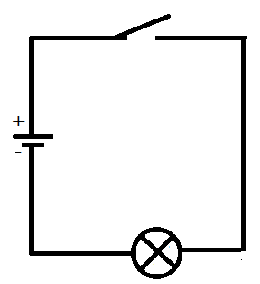
\includegraphics[width=5cm]{circuit}
\centering
\caption{Een circuit}
\label{symbool:circuit}
\end{figure}

De symbolen zoals deze worden weergegeven in de elektronica is waar dit document over gaat.


\section{Geleider}
De lijntjes in een circuit die de verschillende onderdelen met elkaar verbinden kunnen gezien worden als stroomdraden. Stroomdraden zijn over het algemeen gemaakt van koper met daar om heen een plastic laag. Koper is een goede geleider van elektrische stroom. Een geleider\index{Geleider}\index{Conductor} is dus een materiaal dat elektriciteit geleidt. Een geleider wordt gebruikt om bijvoorbeeld stroom vanaf het stopcontact te geleiden naar een lamp.

Geleiders kunnen uit verschillende materialen gemaakt worden. Het meest gebruikte materiaal is koper, maar op computer componenten komt ook goud veel voor.


\section{Isolator}
Een isolator\index{Isolator} is een stof die niet geleidt. Het kan een warmte isolator zijn, maar ook een elektrische isolator. Zo zitten rond de elektriciteitsdraden in huis een plastic mantel, die zorgt ervoor dat je niet in direct contact met de geleider kan komen.


\chapter{Voeding}
\section{Batterij}
Een batterij\index{Batterij}\index{Battery} is een apparaat dat elektrische energie op kan slaan. Het doet dit door gebruik te maken van chemische reacties. Er zijn verschillende soorten batterijen: knoopcellen, staafcellen en accu's.

In de elektronica wordt een batterij weergegeven met het symbool dat je ziet weergegeven in \ref{symbool:battery}

\begin{figure}[h]
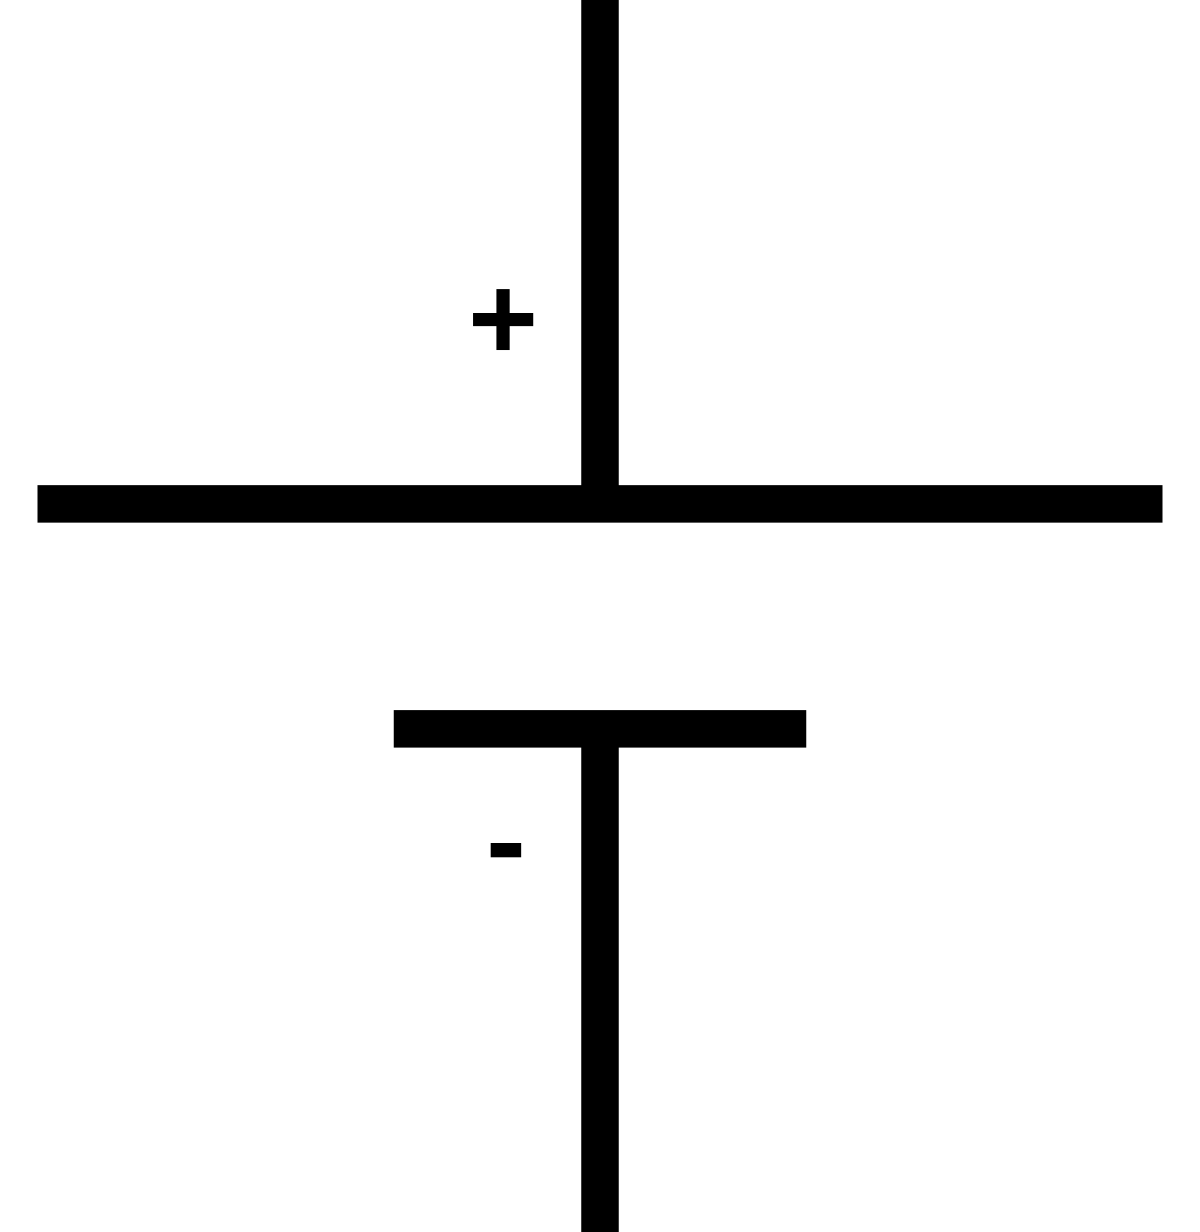
\includegraphics[width=5cm]{batterij}
\centering
\caption{Symbool van een batterij}
\label{symbool:battery}
\end{figure}



\chapter{Gebruikers}
Als we stroom en spanning vergelijken met een rivier dan is het hoogte verschil bepalend voor de snelheid waarmee de rivier zou kunnen stromen. De bodem van de rivier remt het water af, we noemen dat de weerstand. Er zijn nog andere manieren om de rivier af te remmen en dat is door er een schoepenrad in te zetten. Een schoepenrad in de rivier verbruikt het water niet, maar zorgt er wel voor dat de rivier minder hard stroomt. Het schoepenrad gebruikt de rivier om arbeid te verrichten, bijvoorbeeld om graan te malen.

In de electronica kennen we ook gebruikers, of verbruikers. Gebruikers zorgen ervoor dat de stroom minder snel stroomt. Er wordt dus weerstand geboden aan de stroom. We zeggen dan ook dat bijvoorbeeld een lamp die brandt er voor zorgen dat de weerstand verhoogd wordt. Een gebruiker verbruikt geen stroom, maar zorgt er wel voor dat er in het totale circuit minder stroom loopt.


% Requires batterij
\section{Weerstand}
Als we de + en de - van een batterij met elkaar verbinden dat maken we een kortsluiting. Bij een kortsluiting gaat er heel veel stroom lopen, zoveel zelfs dat het plastic om de geleider in brand zou kunnen vliegen. Om te voorkomen dat dat gebeurd moeten we de stroom beperken. Dit doen we door de weerstand\index{Weerstand} te verhogen. De weerstand vermindert de stroom en daardoor ontstaat er geen brand.

Er zijn verschillende manieren om de weerstand te verhogen. We kunnen gebruik maken van een apparaat dat de stroom gebruikt om te werken (bijvoorbeeld een lamp die brandt), maar we kunnen ook een speciaal stukje elektronica gebruiken, genaamd een weerstand\index{Weerstand}\index{Resistor} die als enige functie heeft de weerstand in een circuit te verhogen zodat de stroom beperkt wordt.

In de elektronica wordt een weerstand weergegeven met het symbool dat je ziet weergegeven in \ref{symbool:weerstand}

\begin{figure}[h]
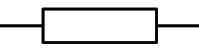
\includegraphics[width=5cm]{weerstand}
\centering
\caption{Symbool van een weerstand}
\label{symbool:weerstand}
\end{figure}


\section{Lamp}
Een lamp\index{Lamp} is \'e\'en van de normaalste zaken in het huishouden. In de elektronica wordt een lamp weergegeven met het symbool dat je ziet weergegeven in \ref{symbool:lamp}

\begin{figure}[h]
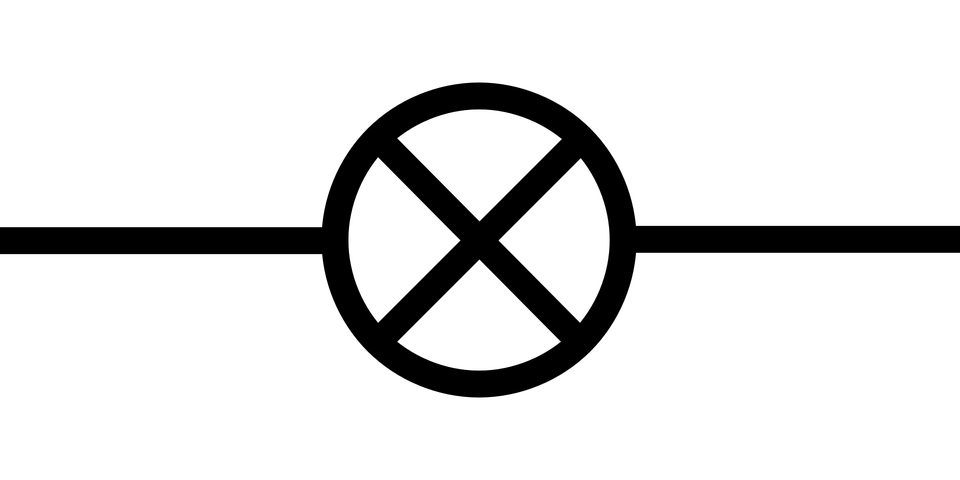
\includegraphics[width=5cm]{lamp}
\centering
\caption{Symbool van een lamp}
\label{symbool:lamp}
\end{figure}


\chapter{Circuit onderbreken}
% Requires: Lamp
\section{Schakelaar}
Een lamp of een andere elektronisch apparaat wil je uit en aan kunnen zetten. Dat schakelen doen we met een schakelaar (Engels: switch)\index{Schakelaar}\index{Switch}.

In de elektronica wordt een switch weergegeven met het symbool dat je ziet weergegeven in \ref{symbool:switch}

\begin{figure}[h]
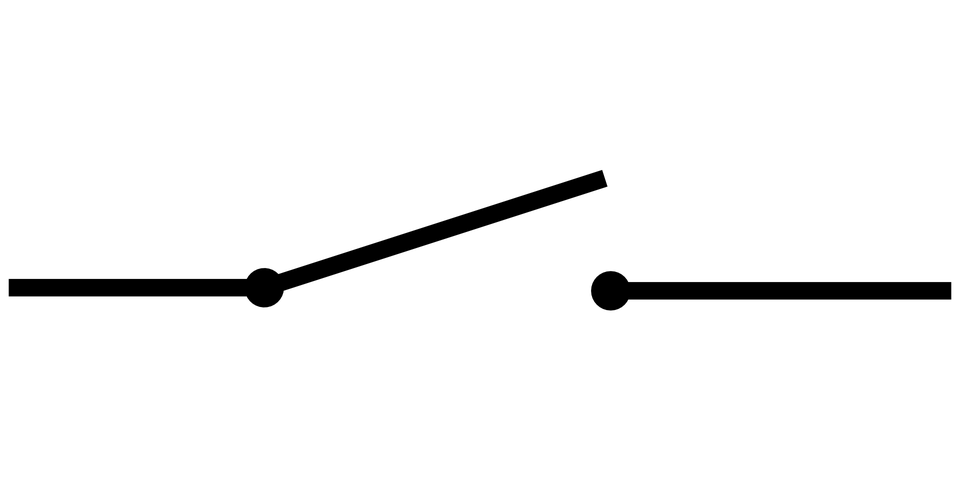
\includegraphics[width=5cm]{switch}
\centering
\caption{Symbool van een schakelaar}
\label{symbool:switch}
\end{figure}

Er zijn verschillende soorten schakelaars en toch zal je over het algemeen alleen het weergegeven symbool voor de schakelaar tegen komen.

% Requires: Schakelaar
\section{Zekering}
Een zekering\index{Zekering}\index{Fuse} is een component dat elektronica of mens en dier beschermt tegen te grote hoeveelheden stroom. Op het moment dat er te veel stroom loopt zal de zekering doorbranden of uitslaan. Een zekering die doorbrandt noemen we een smeltzekering. Een zekering die uitslaat een elektronische zekering, deze werkt dus eigenlijk als een schakelaar.

In de elektronica wordt een zekering weergegeven met het symbool dat je ziet weergegeven in \ref{symbool:fuse}

\begin{figure}[h]
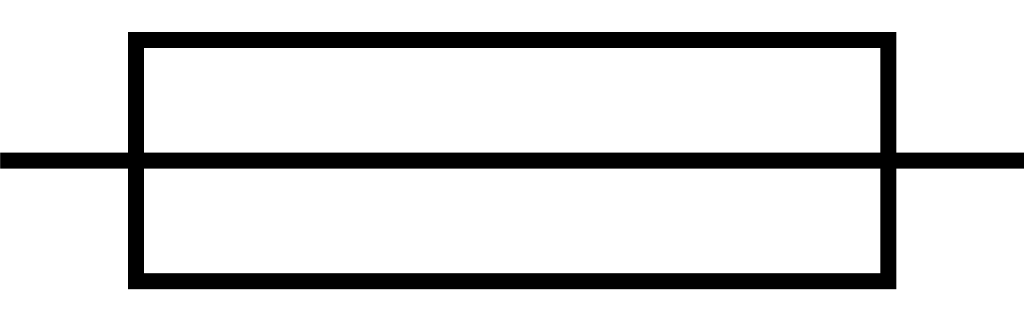
\includegraphics[width=5cm]{fuse}
\centering
\caption{Symbool van een zekering}
\label{symbool:fuse}
\end{figure}

\section{Aardlekschakelaar}
In een circuit moet wat erin gaat er ook uit komen. Als in een formule 1 wedstrijd 18 auto's aan de start verschijnen, dan zou het fijn zijn als er ook 18 auto's aan de finish komen. Mist er een auto dan is er wat fout gegaan. Als in een elektronisch circuit er aan het einde niet meer dezelfde hoeveelheid stroom is als aan het begin dan spreken we van een lek. Lekstromen kunnen gevaarlijk zijn, want het kan betekenen dat een deel van de stroom via een mens een andere route gevonden heeft. Om de mens te beschermen tegen deze stroom is er de aardlekschakelaar\index{Aardlekschakelaar}\index{Earth Leakage Circuit Breaker). Als de elektronica in de schakelaar detecteerd dat er stroom "verdwenen" is dan schakelt de schakelaar het circuit uit.

In de elektronica wordt een aardlekschakelaar weergegeven met het symbool dat je ziet weergegeven in \ref{symbool:aardlekschakelaar}

\begin{figure}[h]
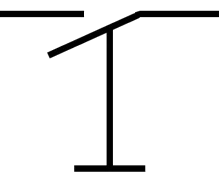
\includegraphics[width=5cm]{aardlekschakelaar}
\centering
\caption{Symbool van een aardlekschakelaar}
\label{symbool:aardlekschakelaar}
\end{figure}



\chapter{Speciale componenten}
% Requires: Weerstand, Isolator, Batterij
\section{Condensator}
Een condensator\index{Condensator}\index{Capacitor} bestaat uit twee platen van een geleidend materiaal dat bescheiden wordt door een isolator, een zogenaamd di\"electricum. Als er een spanning gezet wordt op een circuit met een condensator erin dan zullen de elektronen naar de plus pool willen bewegen, daardoor worden er elektronen aan de plaat die aan de plus pool hangt onttrokken, deze zal dan positief geladen worden. Bij de min-pool gebeurt precies het omgekeerde en de plaat aan de min-pool wordt nu negatief geladen. Koppelen de we batterij los, dan houden we een geladen condensator over, met een spanning die gelijk is aan de spanning batterij.

De hoeveelheid lading die we op een condensator kunnen opslaan is beperkt, dus hij is dan ook zo weer leeg gelopen. Een condensator werkt dus als een mini-batterij.

In de elektronica wordt een condensator weergegeven met het symbool dat je ziet weergegeven in \ref{symbool:condensator}

\begin{figure}[h]
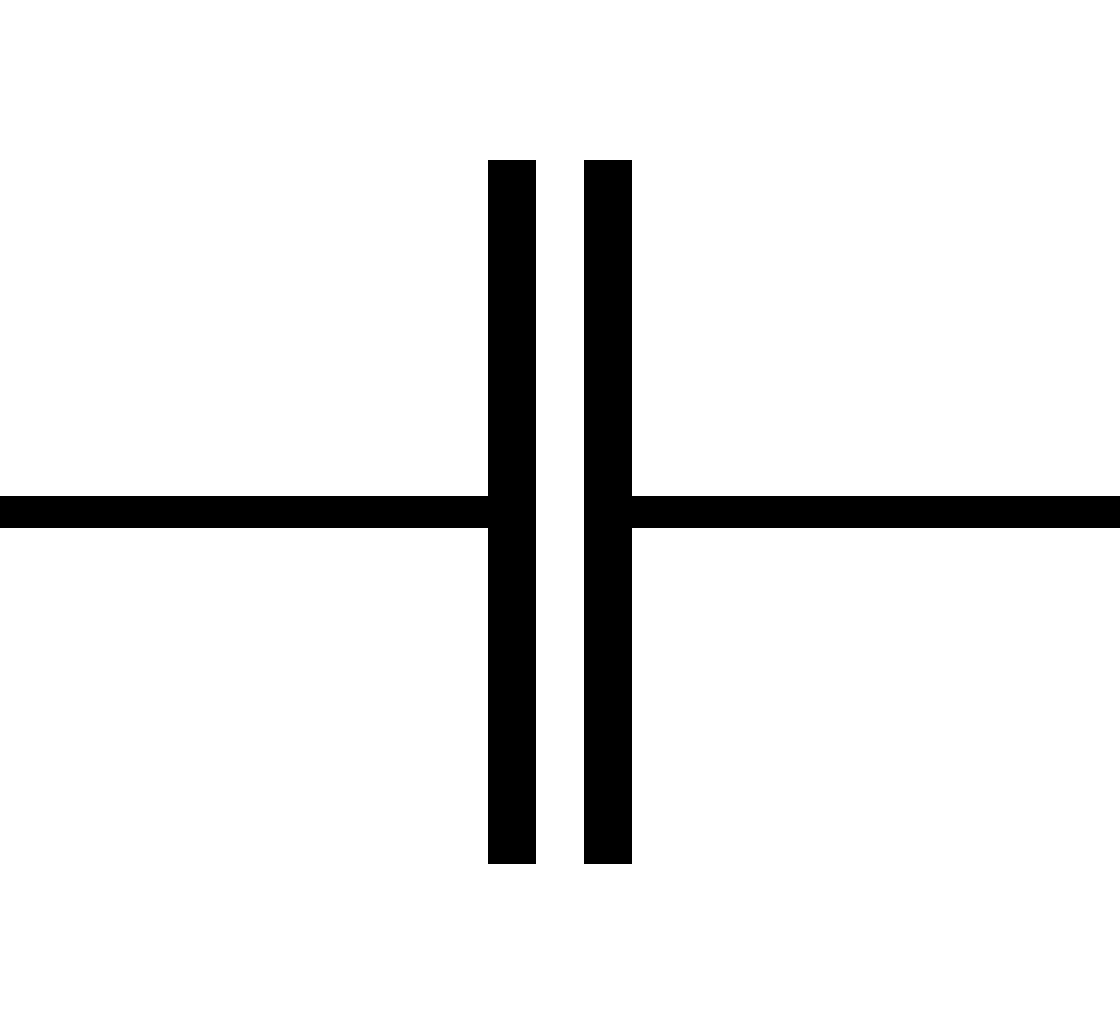
\includegraphics[width=5cm]{condensator}
\centering
\caption{Symbool van een condensator}
\label{symbool:condensator}
\end{figure}


\section{Spoel}
Een spoel\index{Spoel}\index{Coil} is een stuk geleider die opgerold is tot een rolletje.

Als we een spanning zetten op deze spoel van vormt hij een magnetisch veld. Er ontstaat dus een noord-pool en een zuid-pool en hij werkt dan als een, zwakke, magneet.

In de elektronica wordt een switch weergegeven met het symbool dat je ziet weergegeven in \ref{symbool:spoel}

\begin{figure}[h]
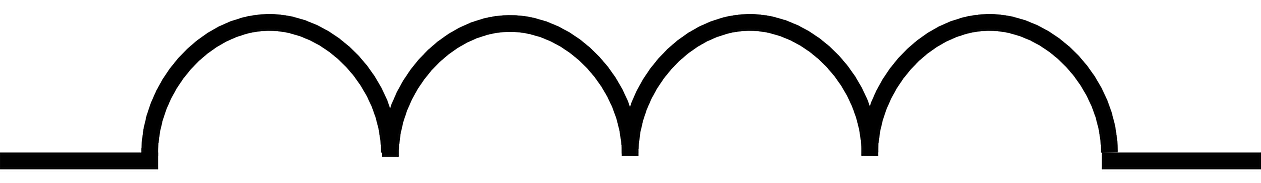
\includegraphics[width=5cm]{spoel}
\centering
\caption{Symbool van een spoel}
\label{symbool:spoel}
\end{figure}

Zetten we een wisselspanning op de spoel dan zullen de noord- en zuidpool wisselen van de ene kant van de spoel naar de andere.


% Requires: Spool
\section{Transformator}
Een voeding van een PC heeft als ingangsspanning 230 Vac en als uitgangsspanning 12, 5, en 3,3 Vdc. De ingangsspanning moet dus omgezet worden naar een gelijkspanning en hij moet omgezet worden van 230 V naar bijvoorbeeld 12 V. Het verlagen van de spanning is de taak van de transformator\index{Transformator}\index{Transformer}. De transformator werkt met de inkomende wisselspanning, dus de uitgaande spanning is bijvoorbeeld 23 Vac.

In de elektronica wordt een transformator weergegeven met het symbool dat je ziet weergegeven in \ref{symbool:transformator}

\begin{figure}[h]
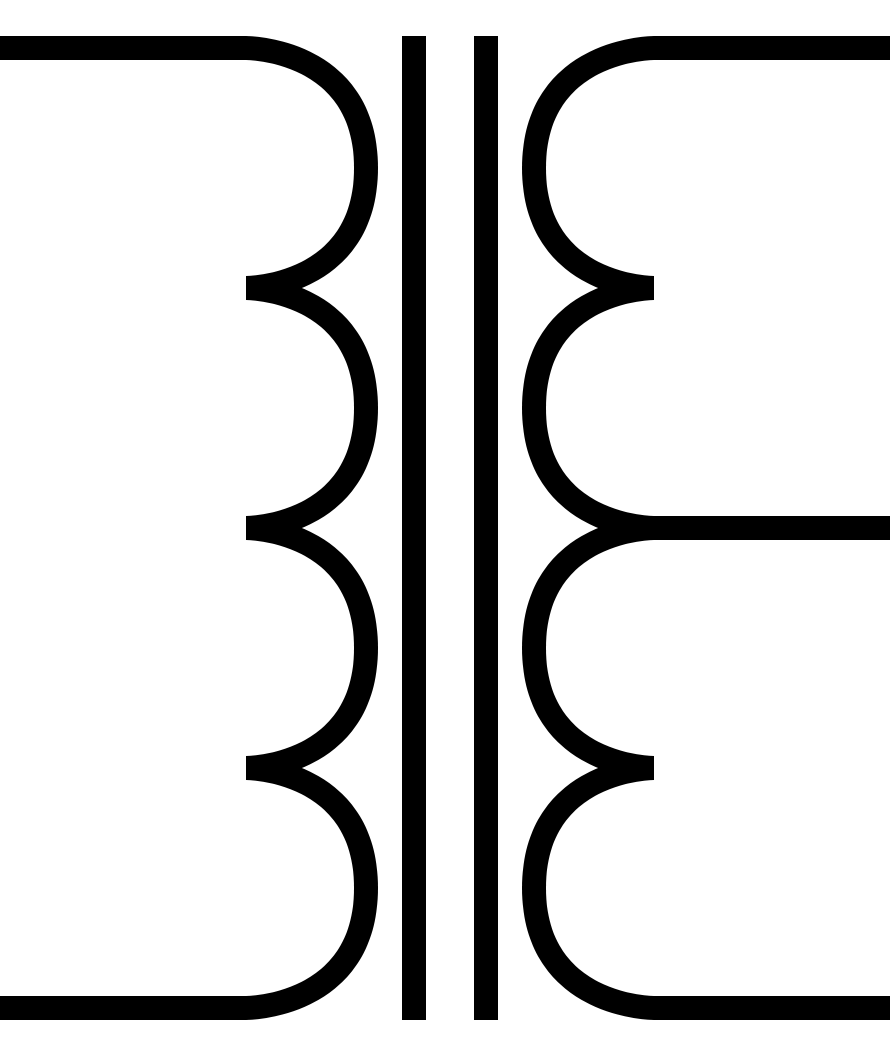
\includegraphics[width=5cm]{transformator}
\centering
\caption{Symbool van een transformator}
\label{symbool:transformator}
\end{figure}

Een transformator bestaat uit twee spoelen die verbonden zijn door een metalen-kern. De kern geleidt het magnetische veld dat door de primaire spoel wordt opgewekt, zie figuur \ref{fig:transformator3D}.

\begin{figure}[h]
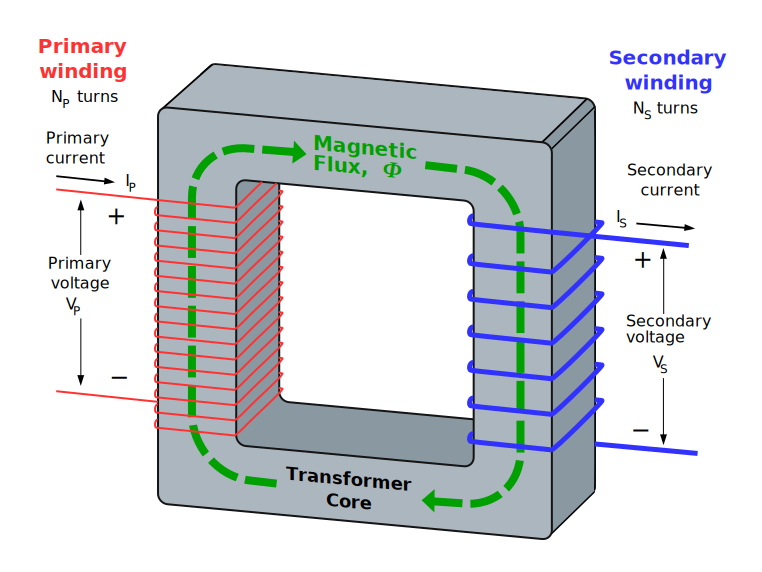
\includegraphics[width=10cm]{Transformer3d-col3}
\centering
\caption{Symbool van een 3D transformator}
\label{fig:transformator3D}
\end{figure}

Door het magnetische veld ontstaat in de tweede spoel een spanning en kan er stroom lopen door het circuit dat aan de tweede spoel gekoppeld zit. Als de primaire en de secundaire spoelen een gelijk aantal windingen hebben dan is de primaire spanning gelijk aan de secundaire spanning. Heeft de primaire spoel twee keer zoveel windingen als de secundaire spoel, dan wordt de spanning verlaagt met de helft. Dus 230 Vac aan de primaire kant wordt dan 115 Vac aan de secundaire kant. Heeft de primaire kant minder wikkelingen dan de secundaire kant dan wordt de spanning verhoogt.

De omrekening van primaire spanning naar secundaire spanning kan gedaan worden via de formule \[ V_s = V_p \frac{N_p}{N_s} \].


\chapter{Halfgeleiders}
\section{Diode}
Een diode\index{Diode} laat stroom door in \'e\'en richting, alleen van de anode (A) naar de kathode (C). Van de kathode naar de anode kan er geen stroom lopen.

In de elektronica wordt een diode weergegeven met het symbool dat je ziet weergegeven in \ref{symbool:diode}

\begin{figure}[h]
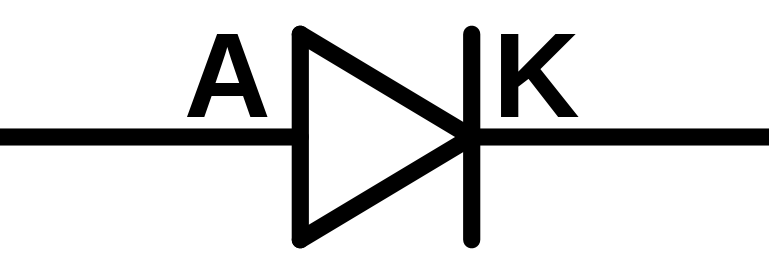
\includegraphics[width=5cm]{diode}
\centering
\caption{Symbool van een diode}
\label{symbool:diode}
\end{figure}

Een diode die licht kan geven noemen we een LED, Light Emitting Diode.

\section{Transistor}
Een transistor\index{Transistor} is een elektronische schakelaar. Door op de 'B-knop', basis, te drukken kan er een stroom lopen van C, collector, naar de E, emittor. De basis wordt 'ingedrukt' door er een spanning op te zetten.

In de elektronica wordt een transistor weergegeven met het symbool dat je ziet weergegeven in \ref{symbool:transistor}

\begin{figure}[h]
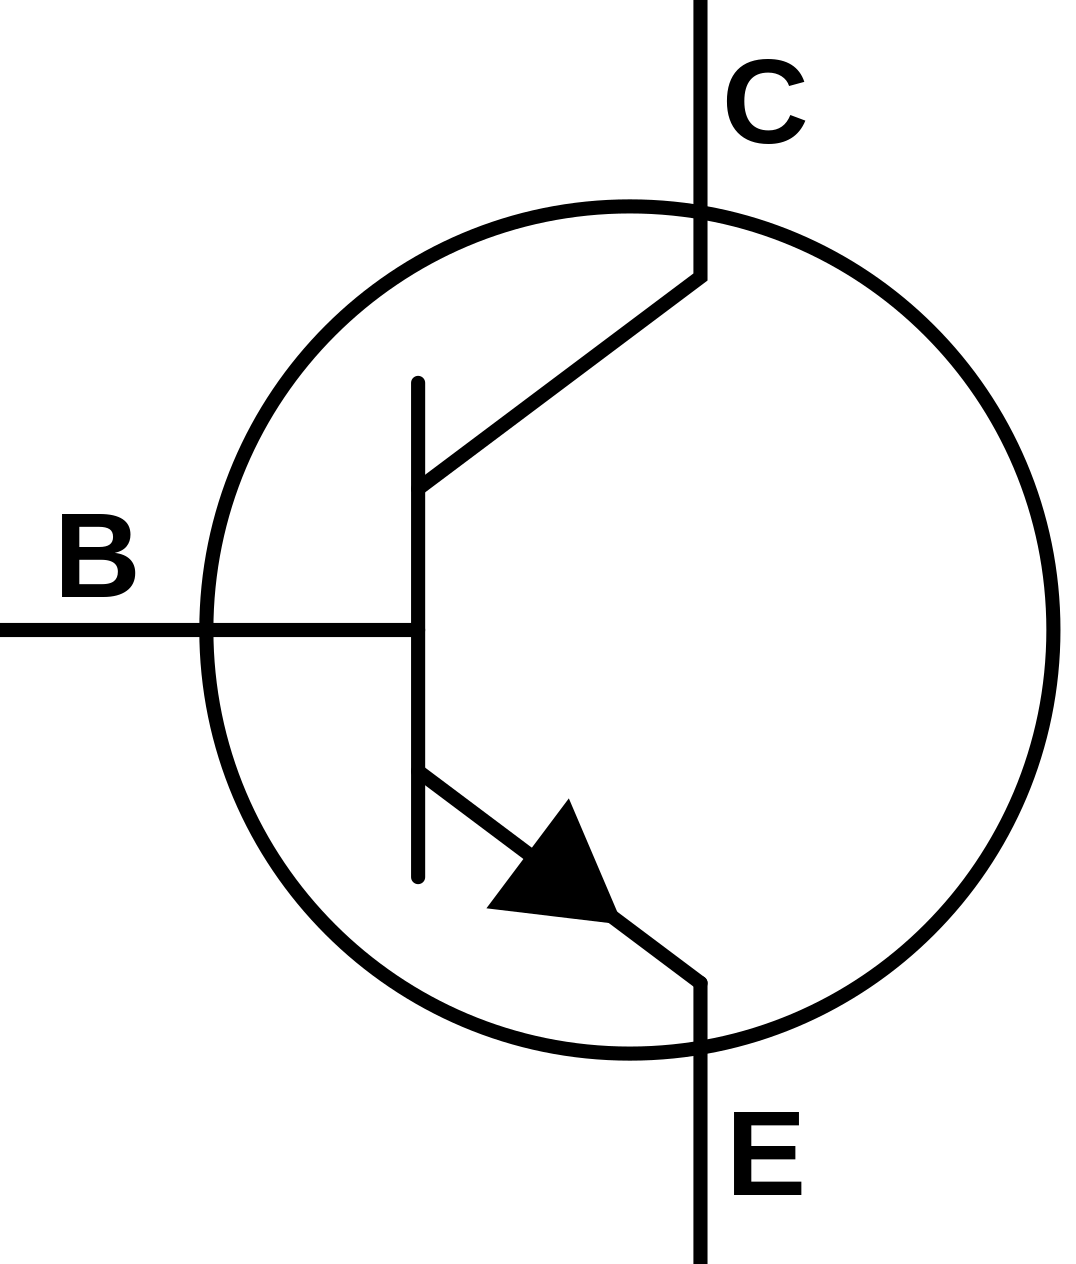
\includegraphics[width=5cm]{transistor}
\centering
\caption{Symbool van een transistor}
\label{symbool:transistor}
\end{figure}




%%%%%%%%%%%%%%%%%%%%%
%%% Index and End %%%
%%%%%%%%%%%%%%%%%%%%%
\backmatter
\printindex
\end{document}

%%% Last line %%%
